\section{System Architecture Design}
\label{VT:Sec:Architecture}

\subsection{System Overview}
Figure~\ref{VT:Fig:ContainerVirtualTime} depicts the architecture of our virtual time system within a Linux-container-based network emulator. 
Linux container~\cite{LXC} is a lightweight virtualization technique that enables multiple instances of Linux OS sharing the kernel. 
Linux container has less overhead than full or para-virtualization platforms, such as Xen, QEMU, or VMware,
in which separated kernels are required for each VM, and therefore,
has been applied in the area of scalable network emulation.
For example, Mininet~\cite{Mininet} is a Linux-container-based emulation platform supporting SDN research. 

Mininet creates containers to virtualize network hosts, and each container has its own private network namespace and interface. 
Applications (such as web services) are encapsulated in the containers. The containers are connected by software switches (typically kernel-model Open vSwitch~\cite{OpenvSwitch}) with virtual interfaces and links as shown in Figure~\ref{VT:Fig:ContainerVirtualTime}, and are multiplexed onto the physical machine. 
Like many other network emulators, Mininet is also vulnerable to the temporal fidelity issue in large-scale network experiments. 
Containers use the same system clock of the physical machine, but the execution of the containers is scheduled by the OS in serial. 
This leads to incorrect perception of time in a container, because the container's clock keeps advancing even if it is not running (e.g., idle, waiting, suspended). 
Such errors are particularly severe when emulating high workload network experiments.

To improve the temporal fidelity, we build a virtual time system as a lightweight middleware in the Linux kernel (see Figure~\ref{VT:Fig:ContainerVirtualTime}). 
We employ the time dilation technique to provide the illusion that a container has as much processing power,
disk I/O, and network bandwidth as a real physical host in a production network despite the fact that it shares the underlying resources with other containers. 
The basic idea is to make time appear to be slower than the wall-clock time, so that the emulated network appears faster.

A capable virtual time system for scalable network emulation needs to have the following requirements:
(1) lightweight design with low system overhead,
(2) transparent virtual time provision to applications in containers, i.e., no code required modification,
(3) universal virtual time support within the emulator and invisible to other processes on the same machine, and
(4) ease of integration to the emulator. 
Accurate and positive emulation results can improve the confidence that any changes
(e.g., a transformation from a traditional network to an SDN-based architecture) to the target production network will be successfully deployed. 

\begin{figure*}
    \centering
    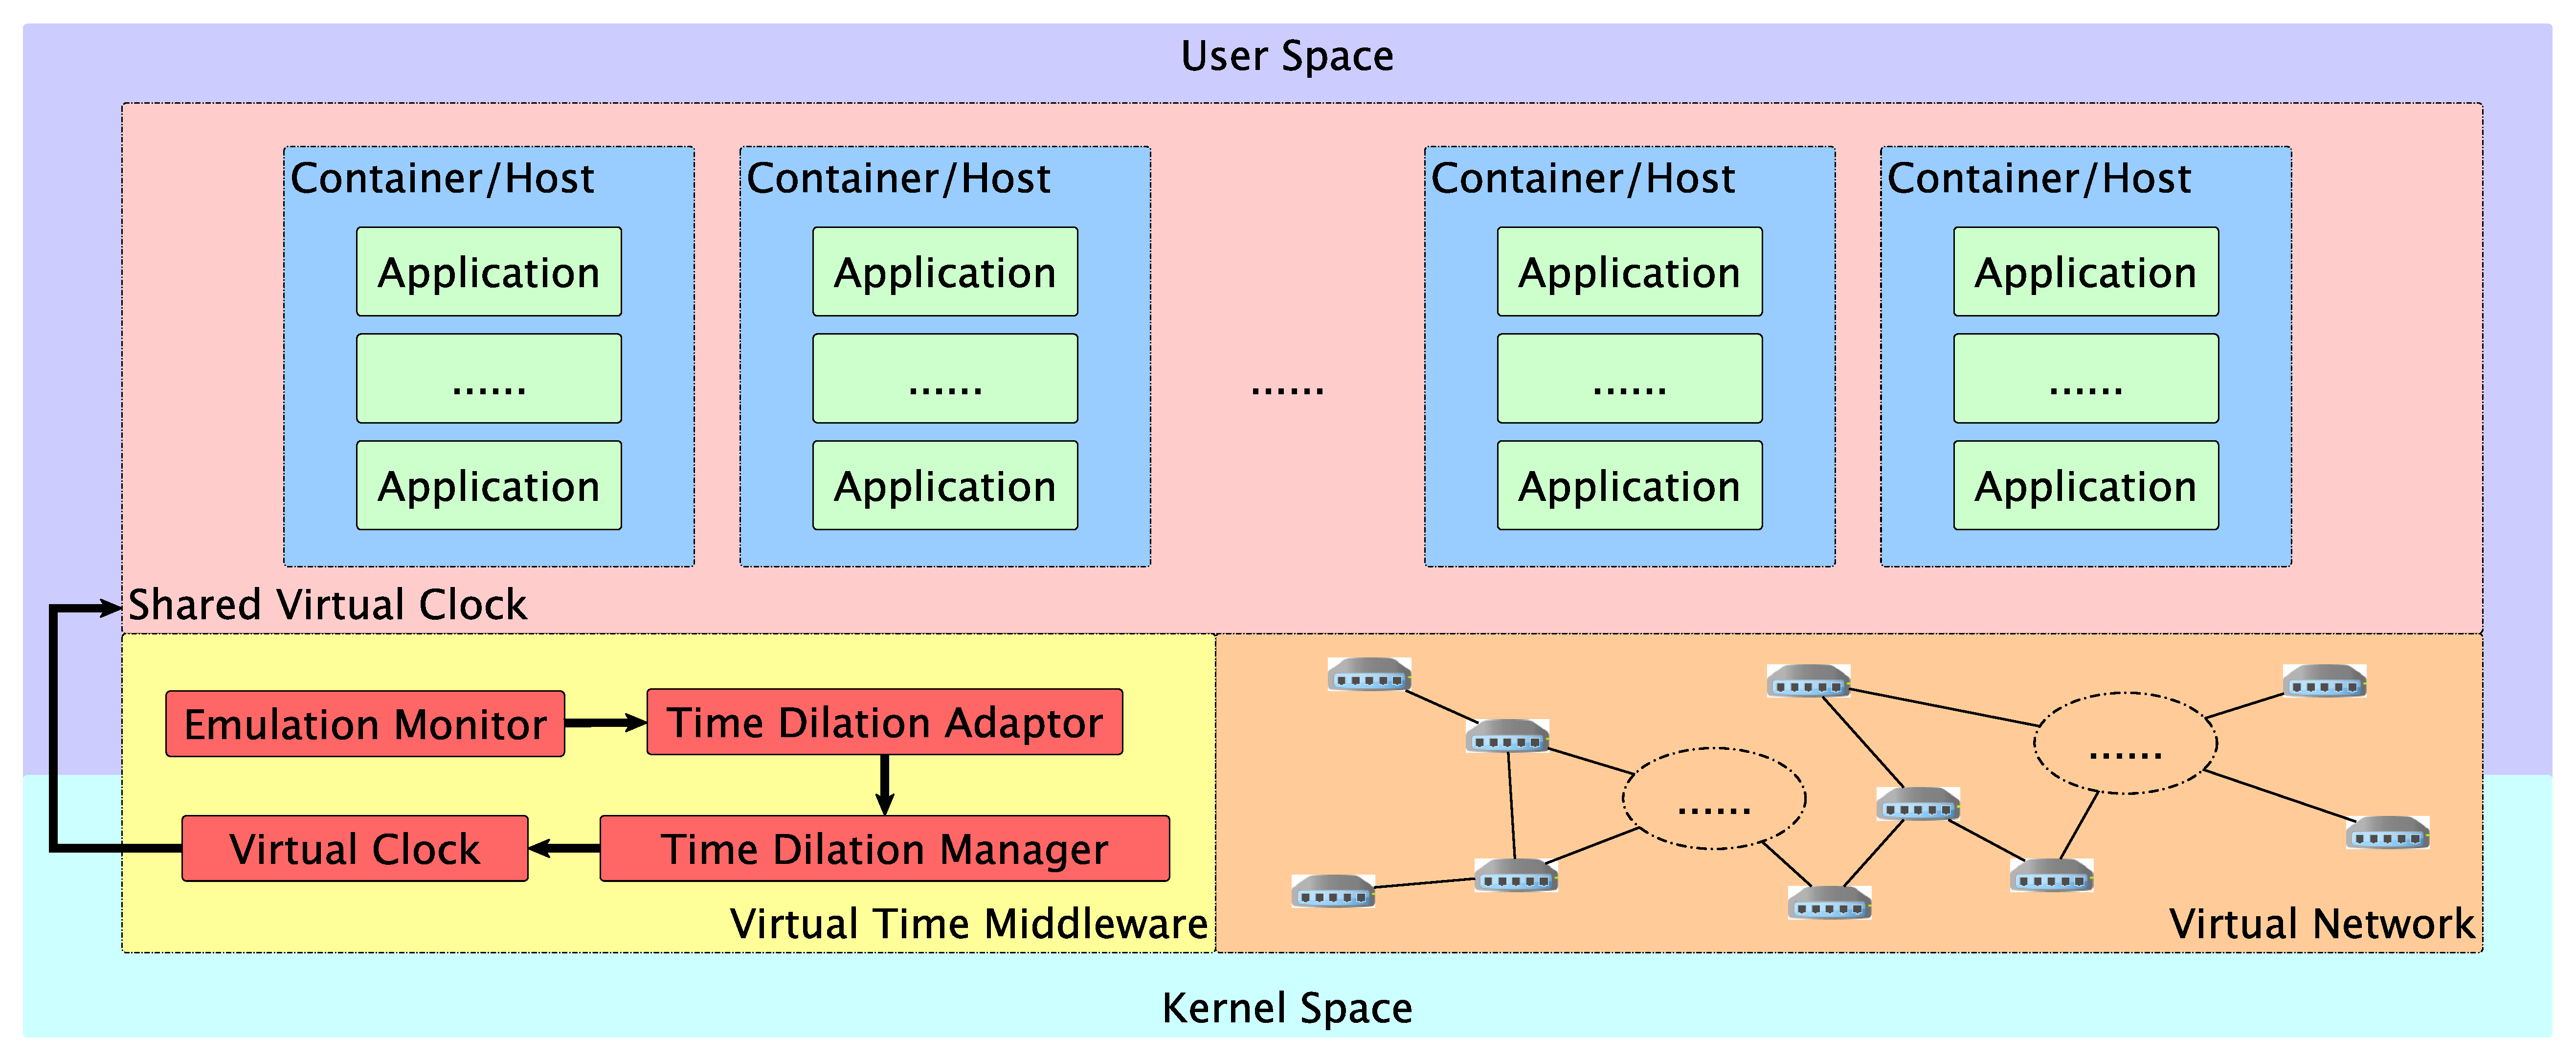
\epsfig{file=VirtualTime/figures/ContainerVirtualTime.eps, height=2in, width=5in}
    \caption[Virtual Time System Design]{Architecture of the Virtual Time System in a Container-based Network Emulator.
    Note that a typical container-based network emulator can be presented by this figure without the Virtual Time Middleware.}
    \label{VT:Fig:ContainerVirtualTime}
\end{figure*}

\Subsection{Virtual Time Management}
Our virtual time system, as shown in Figure~\ref{VT:Fig:ContainerVirtualTime}, is designed to meet all the requirements. 
The time dilation manager is responsible for computing and maintaining the virtual time, according to a given TDF for all the containers. 
It can offer per-container virtual time or the global virtual time for the emulator.
The per-container virtual time is useful to support synchronized emulation (in virtual time) and facilitates the integration with network simulators. 
We have made a small set of changes in the kernel, in particular, a modified data structure to present virtual time,
and a new algorithm to convert the elapsed wall-clock time to the dilated virtual time, with no dependency on third-party libraries.

We attach each container an integer-valued TDF, which could also be shared among all containers. 
A TDF of $k$ slows down a container's time advancement rate by a factor of $k$, thus re-scales a container's notion of time with reference to a physical network. 
This way, Mininet can emulate a seemingly $k$ times faster network owing to the accelerated rate of interaction between the containers and the virtual network
%When TDF is greater than 1, it appears to the containers that available resources including link bandwidth and CPU computation capacity are increased by a factor of TDF. 
Note that our design cannot scale the capacity of hardware components such as main memory, processor caches, and disk, firmware on network interfaces. 

The integration with Mininet, and potentially other container-based software is straightforward. 
We provide a set of simple APIs to (1) initialize containers with virtual time, and (2) inquire virtual time at run time. 
The system returns precise virtual time to container processes and transparently to all their child processes while returning the ordinary system time to other processes. 
We have integrated the system with Mininet. The implementation details are discussed in Section~\ref{VT:Sec:Implementation}, and we have madee our code base available to public on GitHub\footnote{see \href{https://github.com/littlepretty/VirtualTimeForMininet}{VirtualTimeForMininet}}. 

\subsection{Adaptive Time Dilation}
The key insight of virtual time is to trade time with available system resources.
The execution time can be unnecessarily long with an overestimated TDF. 
It is difficult to avoid that with a fixed TDF when the resource demands vary substantially during the emulation. 
Therefore, we investigate means to adaptively adjust TDF in run-time with the goal of well balancing the execution speed and accuracy. 
We take a similar epoch-based approach described in~\cite{NtwkEmultAdaptVirtTime}, and develop two modules,
Emulation Monitor and Time Dilation Adaptor (see Figure~\ref{VT:Fig:ContainerVirtualTime}), to achieve the dynamic TDF adjustment. 

Emulation Monitor periodically collects the process-related information (not necessarily coincides with the epoch duration)
and computes the run-time emulation load statistics, such as CPU utilization, number of waiting processes, or average process waiting time. 
Time Dilation Adaptor takes the inputs from Emulation Monitor, and adaptively computes the TDF for the next epoch based on a heuristic algorithm,
whose details are presented in Section~\ref{VT:Sec:Implementation}. 
Currently we only use the CPU utilization as the feedback control indicator, and will leave the exploration of other control algorithms as future works. 

